\documentclass[11pt]{beamer}
\useoutertheme{infolines}
\setbeamertemplate{headline}

\useinnertheme{default}
\usecolortheme{orchid}


\usepackage[utf8]{inputenc}
\usepackage[english]{babel}
\usepackage{amsmath}
\usepackage{amsfonts}
\usepackage{amssymb}
\usepackage{graphicx}
\graphicspath{{../imgs/}}
\usepackage{hyperref}
\urlstyle{same}

% für subfigure:
\usepackage{caption}
\usepackage{subcaption}
% tikz pakete für die Erstellung von plots:
\usepackage{tikz}
\usepackage{pgfplots}
\pgfplotsset{compat=newest}

\usepackage[
backend=bibtex,
sortcites=false,
style=numeric,
firstinits=true,
uniquename=init,
isbn=false,
pagetracker=false,
maxbibnames=50,
maxcitenames=3,
autocite=inline,
block=space,
backref=false,
backrefstyle=three+,
date=short,
url=false,
doi=true,
eprint=false,
sorting=none
]{biblatex}
\addbibresource{refs.bib}

\usefonttheme[onlymath]{serif}


\author{Markus Hartlage}
\title[Digitaler Funktionsgenerator in VHDL]{Entwicklung und Implementierung eines digitalen Funktionsgenerators in VHDL}
%\setbeamercovered{transparent} 
%\setbeamertemplate{navigation symbols}{} 
\titlegraphic{
\includegraphics[width=3cm]{logo.png}}
\institute{FH-Bielefeld} 
%\date{} 
%\subject{}
\begin{document}

\begin{frame}
\titlepage
\end{frame}

%\begin{frame}
%\tableofcontents
%\end{frame}

% Konzept
% Funktionskomponenten
% Konfiguration - hier kann ich vielleicht das python Interface zeigen
% Funktionstests
% Fazit

\section{Konzept}

\begin{frame}{Konzept - Anforderungen}
  \begin{itemize}
    \item Ausgabe vier verschiedener Funktionsverläufe
      \begin{itemize}
        \item Konstante, Rechteck, Zick-Zack, Rampe
      \end{itemize}
    \item Konfiguration per UART-Schnittstelle
  \end{itemize}

\begin{figure}[h] \centering
  {
    \pgfplotsset{
    xtick={0, 15, 30, 45, 60, 75, 90},
    ytick={0, 0.55, 1.1, 1.65, 2.2, 2.75, 3.3},
    xmin=0, xmax=90,
    ymin=-0.2, ymax=3.5,
    % xlabel=$t$,
    xticklabels={$0$, , $T$, , $2T$, , $3T$,}, % \pgfmathprintnumber{\tick}},
    yticklabels={},
    grid=major,
    width=0.5\textwidth,
    height=0.3\textwidth
  }
  % constant
    \begin{tikzpicture}
      \begin{axis}[yticklabels={$l$, , , , , ,$h$}, ylabel=$U(t)$]
        \addplot[color=blue, line width=1.5pt] coordinates{(0, 3.3)(90, 3.3)};
      \end{axis}
    \end{tikzpicture}
    \label{Concept:Plot:const}
  % square
    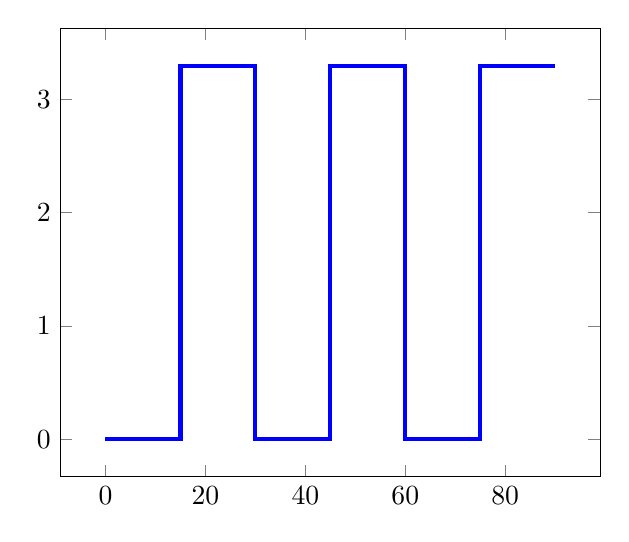
\begin{tikzpicture}
      \begin{axis}
        \addplot[color=blue, line width=1.5pt]  coordinates{(0, 0)(15, 0)(15, 3.3)(30, 3.3)(30, 0)(45, 0)(45, 3.3)(60, 3.3)(60, 0)(75, 0)(75, 3.3)(90, 3.3)};
      \end{axis}
    \end{tikzpicture}
    \label{Concept:Plot:square}

  % zigzag \foreach \x in {0, 15, ..., 90} {(\x, 3.3)}
    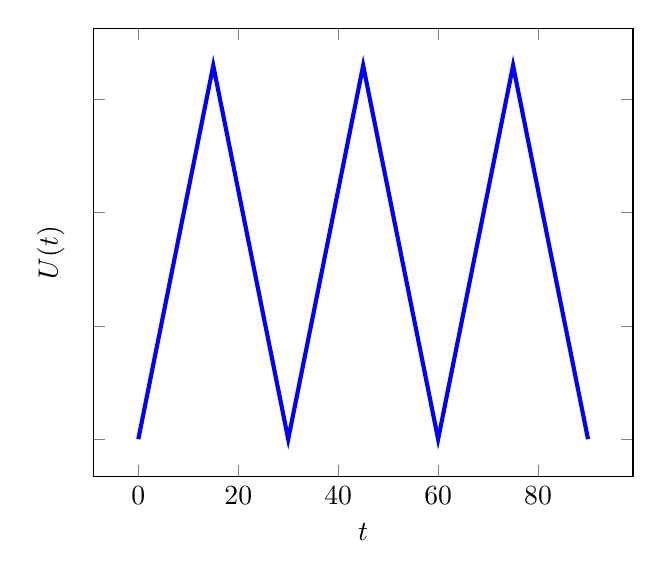
\begin{tikzpicture}
      \begin{axis}[yticklabels={$l$, , , , , ,$h$}, ylabel=$U(t)$, xlabel=$t$]
        \addplot[color=blue, line width=1.5pt] coordinates{(0, 0)(15, 3.3)(30, 0)(45, 3.3)(60, 0)(75, 3.3)(90, 0)};
      \end{axis}
    \end{tikzpicture}
    \label{Concept:Plot:zigzag}
  % ramp
    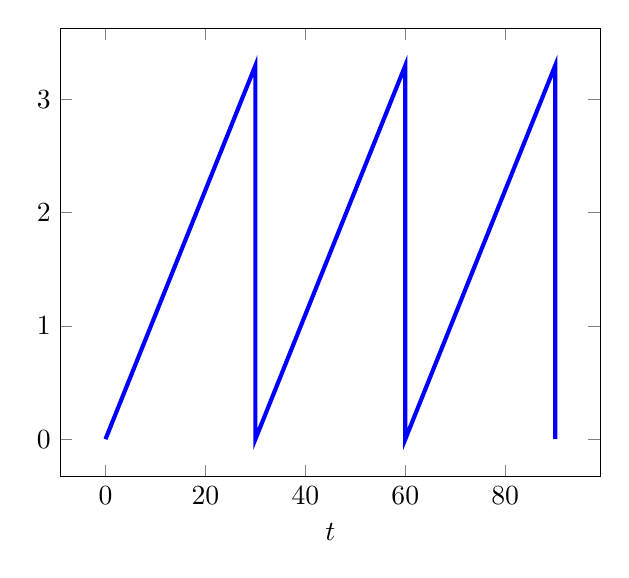
\begin{tikzpicture}
      \begin{axis}[xlabel=$t$]
        \addplot[color=blue, domain=0:90, line width=1.5pt]  coordinates{(0, 0)(30, 3.3)(30, 0)(60, 3.3)(60, 0)(90, 3.3)(90, 0)};
      \end{axis}
    \end{tikzpicture}
    \label{Concept:Plot:ramp}
  }
\end{figure}
  \end{frame}

\begin{frame}{Konzept - Aufbau}
  \begin{itemize}
    \item Aufbau aus Konfigurations-, Funktions- und DAC Komponente
    \item zusätzliche Hardware: Uart-Interface und digital-analog Konverter
  \end{itemize}

  \begin{figure}
    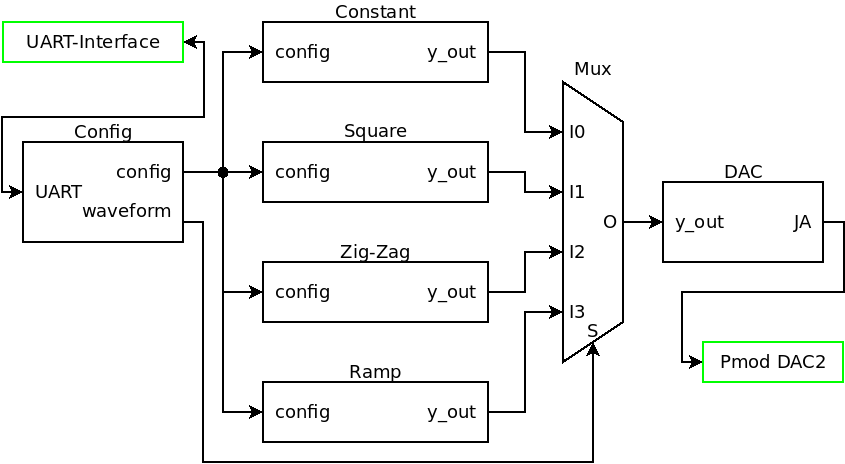
\includegraphics[scale=0.36]{fg_diagram_pres}
  \end{figure}
\end{frame}

\section{Komponenten}

\begin{frame}{Komponenten - Konfiguration}
    Aufbau als state machine:
      \begin{itemize}
        \item Byteweises Einlesen der UART Rx Signale 
        \item Interpretation von vier Bytes als Befehl (Befehlscode + Argumente) 
        \item Berechnung und Speicherung der neuen Konfiguration
      \end{itemize}
  % \begin{figure}
  %   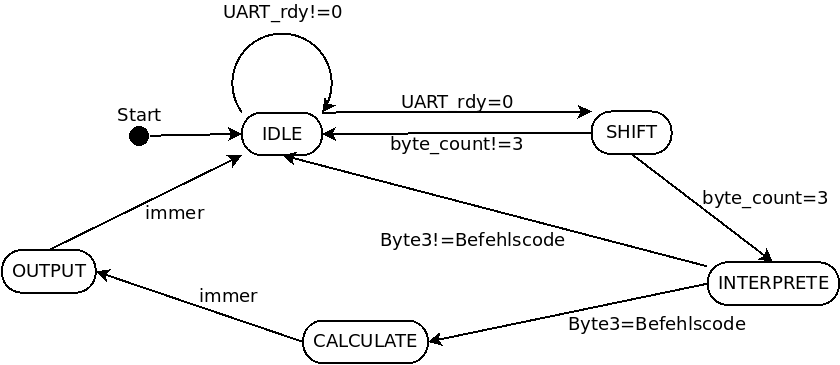
\includegraphics[scale=0.40]{config_state_machine}
  % \end{figure}
      \resizebox{\textwidth}{!}{
      % Graphic for TeX using PGF
% Title: /home/markus/Documents/FH/function_generator_doku/imgs/config_state_machine.dia
% Creator: Dia v0.97+git
% CreationDate: Fri Apr  1 14:09:59 2022
% For: markus
% \usepackage{tikz}
% The following commands are not supported in PSTricks at present
% We define them conditionally, so when they are implemented,
% this pgf file will use them.
\ifx\du\undefined
  \newlength{\du}
\fi
\setlength{\du}{15\unitlength}
\begin{tikzpicture}[even odd rule]
\pgftransformxscale{1.000000}
\pgftransformyscale{-1.000000}
\definecolor{dialinecolor}{rgb}{0.000000, 0.000000, 0.000000}
\pgfsetstrokecolor{dialinecolor}
\pgfsetstrokeopacity{1.000000}
\definecolor{diafillcolor}{rgb}{1.000000, 1.000000, 1.000000}
\pgfsetfillcolor{diafillcolor}
\pgfsetfillopacity{1.000000}
\pgfsetlinewidth{0.100000\du}
\pgfsetdash{}{0pt}
{\pgfsetcornersarced{\pgfpoint{1.000000\du}{1.000000\du}}\definecolor{diafillcolor}{rgb}{1.000000, 1.000000, 1.000000}
\pgfsetfillcolor{diafillcolor}
\pgfsetfillopacity{1.000000}
\fill (20.869812\du,5.684261\du)--(20.869812\du,7.813150\du)--(24.869812\du,7.813150\du)--(24.869812\du,5.684261\du)--cycle;
}{\pgfsetcornersarced{\pgfpoint{1.000000\du}{1.000000\du}}\definecolor{dialinecolor}{rgb}{0.000000, 0.000000, 0.000000}
\pgfsetstrokecolor{dialinecolor}
\pgfsetstrokeopacity{1.000000}
\draw (20.869812\du,5.684261\du)--(20.869812\du,7.813150\du)--(24.869812\du,7.813150\du)--(24.869812\du,5.684261\du)--cycle;
}% setfont left to latex
\definecolor{dialinecolor}{rgb}{0.000000, 0.000000, 0.000000}
\pgfsetstrokecolor{dialinecolor}
\pgfsetstrokeopacity{1.000000}
\definecolor{diafillcolor}{rgb}{0.000000, 0.000000, 0.000000}
\pgfsetfillcolor{diafillcolor}
\pgfsetfillopacity{1.000000}
\node[anchor=base,inner sep=0pt, outer sep=0pt,color=dialinecolor] at (22.869812\du,7.022532\du){IDLE};
\pgfsetlinewidth{0.100000\du}
\pgfsetdash{}{0pt}
{\pgfsetcornersarced{\pgfpoint{1.000000\du}{1.000000\du}}\definecolor{diafillcolor}{rgb}{1.000000, 1.000000, 1.000000}
\pgfsetfillcolor{diafillcolor}
\pgfsetfillopacity{1.000000}
\fill (8.869893\du,12.560686\du)--(8.869893\du,14.689574\du)--(13.551683\du,14.689574\du)--(13.551683\du,12.560686\du)--cycle;
}{\pgfsetcornersarced{\pgfpoint{1.000000\du}{1.000000\du}}\definecolor{dialinecolor}{rgb}{0.000000, 0.000000, 0.000000}
\pgfsetstrokecolor{dialinecolor}
\pgfsetstrokeopacity{1.000000}
\draw (8.869893\du,12.560686\du)--(8.869893\du,14.689574\du)--(13.551683\du,14.689574\du)--(13.551683\du,12.560686\du)--cycle;
}% setfont left to latex
\definecolor{dialinecolor}{rgb}{0.000000, 0.000000, 0.000000}
\pgfsetstrokecolor{dialinecolor}
\pgfsetstrokeopacity{1.000000}
\definecolor{diafillcolor}{rgb}{0.000000, 0.000000, 0.000000}
\pgfsetfillcolor{diafillcolor}
\pgfsetfillopacity{1.000000}
\node[anchor=base,inner sep=0pt, outer sep=0pt,color=dialinecolor] at (11.210788\du,13.898957\du){OUTPUT};
\pgfsetlinewidth{0.100000\du}
\pgfsetdash{}{0pt}
{\pgfsetcornersarced{\pgfpoint{1.000000\du}{1.000000\du}}\definecolor{diafillcolor}{rgb}{1.000000, 1.000000, 1.000000}
\pgfsetfillcolor{diafillcolor}
\pgfsetfillopacity{1.000000}
\fill (44.158474\du,13.173233\du)--(44.158474\du,15.302121\du)--(50.715974\du,15.302121\du)--(50.715974\du,13.173233\du)--cycle;
}{\pgfsetcornersarced{\pgfpoint{1.000000\du}{1.000000\du}}\definecolor{dialinecolor}{rgb}{0.000000, 0.000000, 0.000000}
\pgfsetstrokecolor{dialinecolor}
\pgfsetstrokeopacity{1.000000}
\draw (44.158474\du,13.173233\du)--(44.158474\du,15.302121\du)--(50.715974\du,15.302121\du)--(50.715974\du,13.173233\du)--cycle;
}% setfont left to latex
\definecolor{dialinecolor}{rgb}{0.000000, 0.000000, 0.000000}
\pgfsetstrokecolor{dialinecolor}
\pgfsetstrokeopacity{1.000000}
\definecolor{diafillcolor}{rgb}{0.000000, 0.000000, 0.000000}
\pgfsetfillcolor{diafillcolor}
\pgfsetfillopacity{1.000000}
\node[anchor=base,inner sep=0pt, outer sep=0pt,color=dialinecolor] at (47.437224\du,14.511504\du){INTERPRETE};
\pgfsetlinewidth{0.100000\du}
\pgfsetdash{}{0pt}
{\pgfsetcornersarced{\pgfpoint{1.000000\du}{1.000000\du}}\definecolor{diafillcolor}{rgb}{1.000000, 1.000000, 1.000000}
\pgfsetfillcolor{diafillcolor}
\pgfsetfillopacity{1.000000}
\fill (38.346874\du,5.630771\du)--(38.346874\du,7.759660\du)--(42.346874\du,7.759660\du)--(42.346874\du,5.630771\du)--cycle;
}{\pgfsetcornersarced{\pgfpoint{1.000000\du}{1.000000\du}}\definecolor{dialinecolor}{rgb}{0.000000, 0.000000, 0.000000}
\pgfsetstrokecolor{dialinecolor}
\pgfsetstrokeopacity{1.000000}
\draw (38.346874\du,5.630771\du)--(38.346874\du,7.759660\du)--(42.346874\du,7.759660\du)--(42.346874\du,5.630771\du)--cycle;
}% setfont left to latex
\definecolor{dialinecolor}{rgb}{0.000000, 0.000000, 0.000000}
\pgfsetstrokecolor{dialinecolor}
\pgfsetstrokeopacity{1.000000}
\definecolor{diafillcolor}{rgb}{0.000000, 0.000000, 0.000000}
\pgfsetfillcolor{diafillcolor}
\pgfsetfillopacity{1.000000}
\node[anchor=base,inner sep=0pt, outer sep=0pt,color=dialinecolor] at (40.346874\du,6.969043\du){SHIFT};
\pgfsetlinewidth{0.100000\du}
\pgfsetdash{}{0pt}
{\pgfsetcornersarced{\pgfpoint{1.000000\du}{1.000000\du}}\definecolor{diafillcolor}{rgb}{1.000000, 1.000000, 1.000000}
\pgfsetfillcolor{diafillcolor}
\pgfsetfillopacity{1.000000}
\fill (23.926163\du,16.086808\du)--(23.926163\du,18.215697\du)--(30.161163\du,18.215697\du)--(30.161163\du,16.086808\du)--cycle;
}{\pgfsetcornersarced{\pgfpoint{1.000000\du}{1.000000\du}}\definecolor{dialinecolor}{rgb}{0.000000, 0.000000, 0.000000}
\pgfsetstrokecolor{dialinecolor}
\pgfsetstrokeopacity{1.000000}
\draw (23.926163\du,16.086808\du)--(23.926163\du,18.215697\du)--(30.161163\du,18.215697\du)--(30.161163\du,16.086808\du)--cycle;
}% setfont left to latex
\definecolor{dialinecolor}{rgb}{0.000000, 0.000000, 0.000000}
\pgfsetstrokecolor{dialinecolor}
\pgfsetstrokeopacity{1.000000}
\definecolor{diafillcolor}{rgb}{0.000000, 0.000000, 0.000000}
\pgfsetfillcolor{diafillcolor}
\pgfsetfillopacity{1.000000}
\node[anchor=base,inner sep=0pt, outer sep=0pt,color=dialinecolor] at (27.043663\du,17.425079\du){CALCULATE};
\pgfsetlinewidth{0.100000\du}
\pgfsetdash{}{0pt}
\definecolor{diafillcolor}{rgb}{0.000000, 0.000000, 0.000000}
\pgfsetfillcolor{diafillcolor}
\pgfsetfillopacity{1.000000}
\pgfpathellipse{\pgfpoint{15.725894\du}{6.854147\du}}{\pgfpoint{0.500000\du}{0\du}}{\pgfpoint{0\du}{0.500000\du}}
\pgfusepath{fill}
\pgfsetlinewidth{0.100000\du}
\pgfsetdash{}{0pt}
\pgfsetbuttcap
{
\definecolor{diafillcolor}{rgb}{0.000000, 0.000000, 0.000000}
\pgfsetfillcolor{diafillcolor}
\pgfsetfillopacity{1.000000}
% was here!!!
\pgfsetarrowsend{stealth}
\definecolor{dialinecolor}{rgb}{0.000000, 0.000000, 0.000000}
\pgfsetstrokecolor{dialinecolor}
\pgfsetstrokeopacity{1.000000}
\draw (24.869812\du,5.684261\du)--(38.346874\du,5.630771\du);
}
% setfont left to latex
\definecolor{dialinecolor}{rgb}{0.000000, 0.000000, 0.000000}
\pgfsetstrokecolor{dialinecolor}
\pgfsetstrokeopacity{1.000000}
\definecolor{diafillcolor}{rgb}{0.000000, 0.000000, 0.000000}
\pgfsetfillcolor{diafillcolor}
\pgfsetfillopacity{1.000000}
\node[anchor=base,inner sep=0pt, outer sep=0pt,color=dialinecolor] at (31.608343\du,5.444530\du){UART\_rdy=0};
% setfont left to latex
\definecolor{dialinecolor}{rgb}{0.000000, 0.000000, 0.000000}
\pgfsetstrokecolor{dialinecolor}
\pgfsetstrokeopacity{1.000000}
\definecolor{diafillcolor}{rgb}{0.000000, 0.000000, 0.000000}
\pgfsetfillcolor{diafillcolor}
\pgfsetfillopacity{1.000000}
\node[anchor=base west,inner sep=0pt,outer sep=0pt,color=dialinecolor] at (43.892049\du,10.253461\du){byte\_count=3};
\pgfsetlinewidth{0.100000\du}
\pgfsetdash{}{0pt}
\pgfsetbuttcap
{
\definecolor{diafillcolor}{rgb}{0.000000, 0.000000, 0.000000}
\pgfsetfillcolor{diafillcolor}
\pgfsetfillopacity{1.000000}
% was here!!!
\pgfsetarrowsend{stealth}
\definecolor{dialinecolor}{rgb}{0.000000, 0.000000, 0.000000}
\pgfsetstrokecolor{dialinecolor}
\pgfsetstrokeopacity{1.000000}
\draw (40.346874\du,7.759660\du)--(47.437224\du,13.173233\du);
}
% setfont left to latex
\definecolor{dialinecolor}{rgb}{0.000000, 0.000000, 0.000000}
\pgfsetstrokecolor{dialinecolor}
\pgfsetstrokeopacity{1.000000}
\definecolor{diafillcolor}{rgb}{0.000000, 0.000000, 0.000000}
\pgfsetfillcolor{diafillcolor}
\pgfsetfillopacity{1.000000}
\node[anchor=base west,inner sep=0pt,outer sep=0pt,color=dialinecolor] at (37.159818\du,16.559018\du){Byte3=Befehlscode};
\pgfsetlinewidth{0.100000\du}
\pgfsetdash{}{0pt}
\pgfsetbuttcap
{
\definecolor{diafillcolor}{rgb}{0.000000, 0.000000, 0.000000}
\pgfsetfillcolor{diafillcolor}
\pgfsetfillopacity{1.000000}
% was here!!!
\pgfsetarrowsend{stealth}
\definecolor{dialinecolor}{rgb}{0.000000, 0.000000, 0.000000}
\pgfsetstrokecolor{dialinecolor}
\pgfsetstrokeopacity{1.000000}
\draw (44.158474\du,14.237677\du)--(30.161163\du,17.151252\du);
}
\pgfsetlinewidth{0.100000\du}
\pgfsetdash{}{0pt}
\pgfsetbuttcap
{
\definecolor{diafillcolor}{rgb}{0.000000, 0.000000, 0.000000}
\pgfsetfillcolor{diafillcolor}
\pgfsetfillopacity{1.000000}
% was here!!!
\pgfsetarrowsend{stealth}
\definecolor{dialinecolor}{rgb}{0.000000, 0.000000, 0.000000}
\pgfsetstrokecolor{dialinecolor}
\pgfsetstrokeopacity{1.000000}
\draw (38.346874\du,6.695216\du)--(24.869812\du,6.748705\du);
}
% setfont left to latex
\definecolor{dialinecolor}{rgb}{0.000000, 0.000000, 0.000000}
\pgfsetstrokecolor{dialinecolor}
\pgfsetstrokeopacity{1.000000}
\definecolor{diafillcolor}{rgb}{0.000000, 0.000000, 0.000000}
\pgfsetfillcolor{diafillcolor}
\pgfsetfillopacity{1.000000}
\node[anchor=base,inner sep=0pt, outer sep=0pt,color=dialinecolor] at (31.608343\du,7.560232\du){byte\_count!=3};
\pgfsetlinewidth{0.100000\du}
\pgfsetdash{}{0pt}
\pgfsetbuttcap
{
\definecolor{diafillcolor}{rgb}{0.000000, 0.000000, 0.000000}
\pgfsetfillcolor{diafillcolor}
\pgfsetfillopacity{1.000000}
% was here!!!
\pgfsetarrowsend{stealth}
\definecolor{dialinecolor}{rgb}{0.000000, 0.000000, 0.000000}
\pgfsetstrokecolor{dialinecolor}
\pgfsetstrokeopacity{1.000000}
\draw (44.111387\du,13.367950\du)--(22.869812\du,7.813150\du);
}
% setfont left to latex
\definecolor{dialinecolor}{rgb}{0.000000, 0.000000, 0.000000}
\pgfsetstrokecolor{dialinecolor}
\pgfsetstrokeopacity{1.000000}
\definecolor{diafillcolor}{rgb}{0.000000, 0.000000, 0.000000}
\pgfsetfillcolor{diafillcolor}
\pgfsetfillopacity{1.000000}
\node[anchor=base east,inner sep=0pt, outer sep=0pt,color=dialinecolor] at (37.030862\du,12.354622\du){Byte3!=Befehlscode};
\pgfsetlinewidth{0.100000\du}
\pgfsetdash{}{0pt}
\pgfsetbuttcap
{
\definecolor{diafillcolor}{rgb}{0.000000, 0.000000, 0.000000}
\pgfsetfillcolor{diafillcolor}
\pgfsetfillopacity{1.000000}
% was here!!!
\pgfsetarrowsend{stealth}
\definecolor{dialinecolor}{rgb}{0.000000, 0.000000, 0.000000}
\pgfsetstrokecolor{dialinecolor}
\pgfsetstrokeopacity{1.000000}
\draw (23.926163\du,17.151252\du)--(13.551683\du,13.625130\du);
}
\pgfsetlinewidth{0.100000\du}
\pgfsetdash{}{0pt}
\pgfsetbuttcap
{
\definecolor{diafillcolor}{rgb}{0.000000, 0.000000, 0.000000}
\pgfsetfillcolor{diafillcolor}
\pgfsetfillopacity{1.000000}
% was here!!!
\pgfsetarrowsend{stealth}
\definecolor{dialinecolor}{rgb}{0.000000, 0.000000, 0.000000}
\pgfsetstrokecolor{dialinecolor}
\pgfsetstrokeopacity{1.000000}
\draw (11.210788\du,12.560686\du)--(20.869812\du,7.813150\du);
}
\pgfsetlinewidth{0.100000\du}
\pgfsetdash{}{0pt}
\pgfsetbuttcap
{
\definecolor{diafillcolor}{rgb}{0.000000, 0.000000, 0.000000}
\pgfsetfillcolor{diafillcolor}
\pgfsetfillopacity{1.000000}
% was here!!!
\pgfsetarrowsend{stealth}
\definecolor{dialinecolor}{rgb}{0.000000, 0.000000, 0.000000}
\pgfsetstrokecolor{dialinecolor}
\pgfsetstrokeopacity{1.000000}
\draw (16.274696\du,6.842897\du)--(20.869812\du,6.748705\du);
}
% setfont left to latex
\definecolor{dialinecolor}{rgb}{0.000000, 0.000000, 0.000000}
\pgfsetstrokecolor{dialinecolor}
\pgfsetstrokeopacity{1.000000}
\definecolor{diafillcolor}{rgb}{0.000000, 0.000000, 0.000000}
\pgfsetfillcolor{diafillcolor}
\pgfsetfillopacity{1.000000}
\node[anchor=base west,inner sep=0pt,outer sep=0pt,color=dialinecolor] at (18.738923\du,15.175205\du){immer};
% setfont left to latex
\definecolor{dialinecolor}{rgb}{0.000000, 0.000000, 0.000000}
\pgfsetstrokecolor{dialinecolor}
\pgfsetstrokeopacity{1.000000}
\definecolor{diafillcolor}{rgb}{0.000000, 0.000000, 0.000000}
\pgfsetfillcolor{diafillcolor}
\pgfsetfillopacity{1.000000}
\node[anchor=base west,inner sep=0pt,outer sep=0pt,color=dialinecolor] at (16.040300\du,11.025189\du){immer};
\pgfsetlinewidth{0.100000\du}
\pgfsetdash{}{0pt}
\pgfsetbuttcap
{
\definecolor{diafillcolor}{rgb}{0.000000, 0.000000, 0.000000}
\pgfsetfillcolor{diafillcolor}
\pgfsetfillopacity{1.000000}
% was here!!!
\pgfsetarrowsend{stealth}
\definecolor{dialinecolor}{rgb}{0.000000, 0.000000, 0.000000}
\pgfsetstrokecolor{dialinecolor}
\pgfsetstrokeopacity{1.000000}
\pgfpathmoveto{\pgfpoint{22.754953\du}{5.612562\du}}
\pgfpatharc{396}{139}{1.213226\du and 1.213226\du}
\pgfusepath{stroke}
}
% setfont left to latex
\definecolor{dialinecolor}{rgb}{0.000000, 0.000000, 0.000000}
\pgfsetstrokecolor{dialinecolor}
\pgfsetstrokeopacity{1.000000}
\definecolor{diafillcolor}{rgb}{0.000000, 0.000000, 0.000000}
\pgfsetfillcolor{diafillcolor}
\pgfsetfillopacity{1.000000}
\node[anchor=base,inner sep=0pt, outer sep=0pt,color=dialinecolor] at (21.654934\du,3.407675\du){UART\_rdy!=0};
% setfont left to latex
\definecolor{dialinecolor}{rgb}{0.000000, 0.000000, 0.000000}
\pgfsetstrokecolor{dialinecolor}
\pgfsetstrokeopacity{1.000000}
\definecolor{diafillcolor}{rgb}{0.000000, 0.000000, 0.000000}
\pgfsetfillcolor{diafillcolor}
\pgfsetfillopacity{1.000000}
\node[anchor=base,inner sep=0pt, outer sep=0pt,color=dialinecolor] at (15.725894\du,6.088598\du){Start};
\end{tikzpicture}

}
\end{frame}

\begin{frame}{Komponenten - Square}
  \begin{itemize}
    \item nach 64 steigenden Flanken \emph{Counter} aktivieren
    \item Ausgang auf \emph{low} wenn \emph{o\_count} $>$ \emph{thresh}, sonst \emph{high} 
  \end{itemize}
  \begin{figure}
    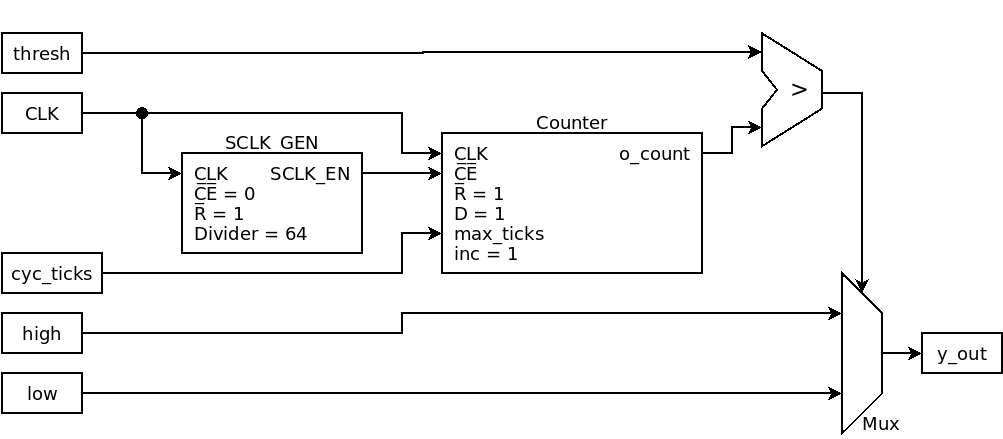
\includegraphics[scale=0.28]{square}
  \end{figure}
\end{frame}

\begin{frame}{Komponenten - Rampe}
  \begin{itemize}
  \item  Abzählen von 64 Taktzyklen
  \end{itemize}
  \begin{figure}
    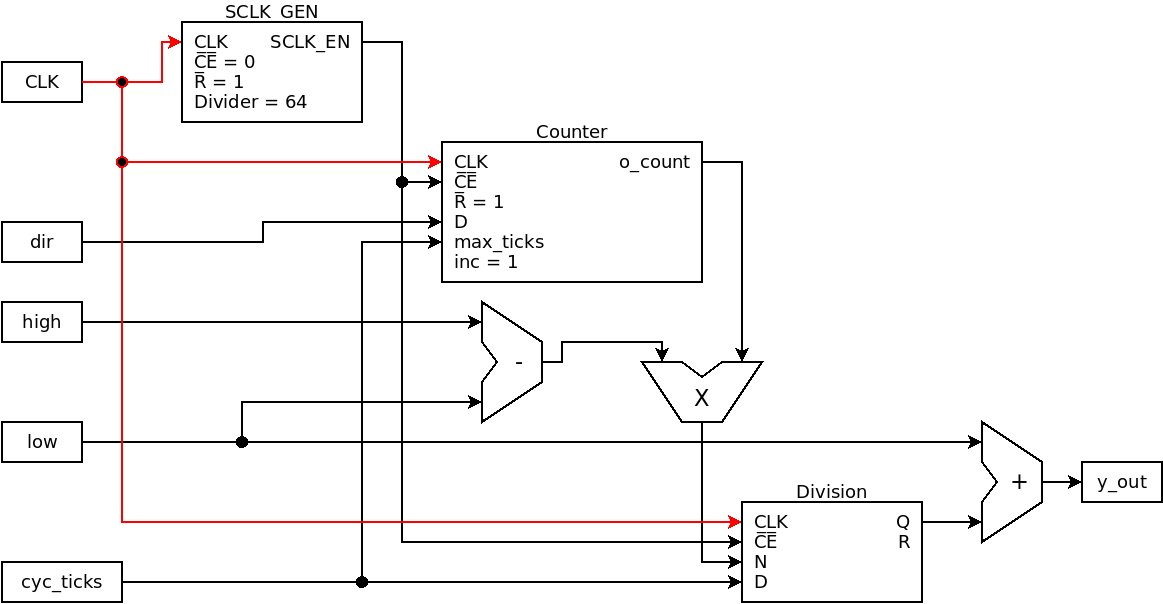
\includegraphics[scale=0.28]{ramp_step0}
  \end{figure}
\end{frame}

\begin{frame}{Komponenten - Rampe}
  \begin{itemize}
    \item Aktivieren des Zählers
  \end{itemize}
  \begin{figure}
    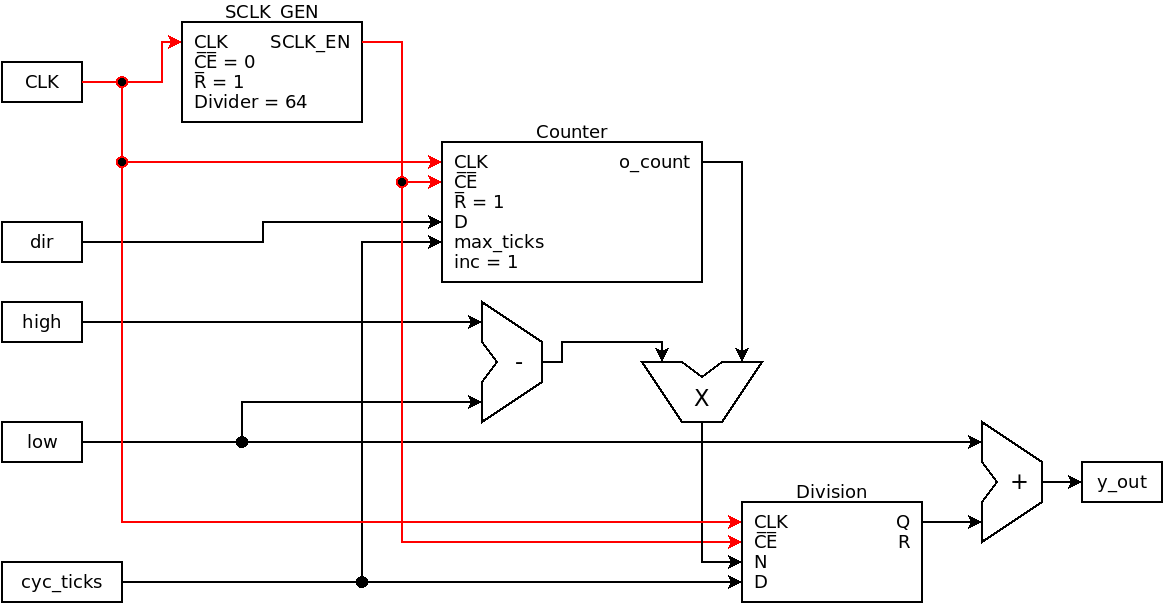
\includegraphics[scale=0.28]{ramp_step1}
  \end{figure}
\end{frame}

\begin{frame}{Komponenten - Rampe}
  \begin{itemize}
    \item neuer Zählstand wird mit Amplitude multipliziert und \emph{Division} beginnt zu teilen
  \end{itemize}
  \begin{figure}
    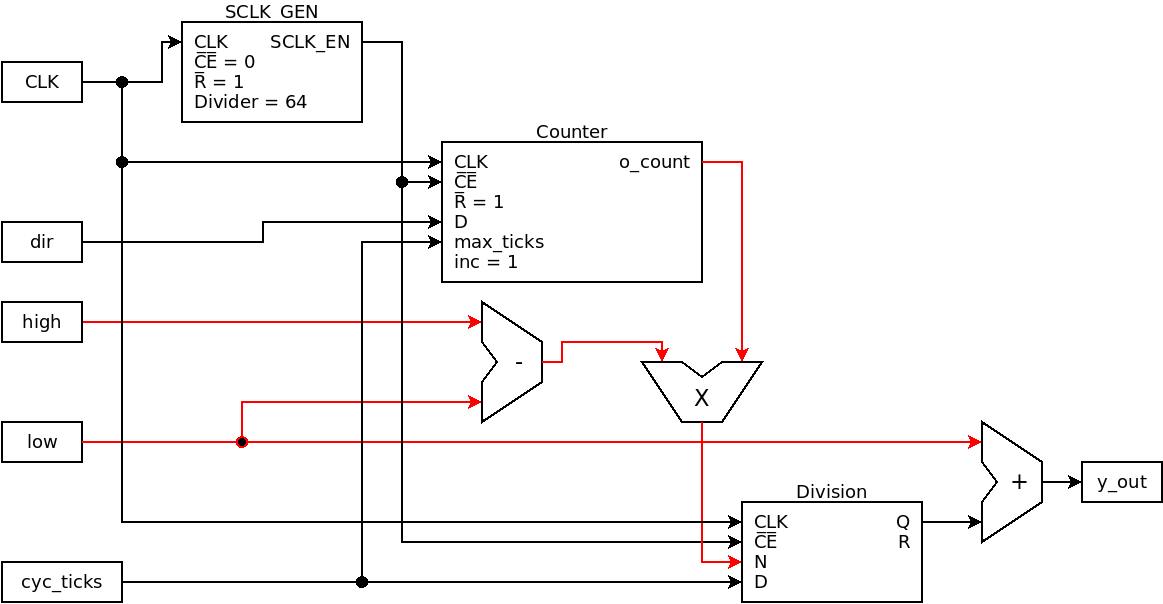
\includegraphics[scale=0.28]{ramp_step2}
  \end{figure}
\end{frame}

\begin{frame}{Komponenten - Rampe}
  \begin{itemize}
    \item untere zwölf Bits von \emph{Q} plus \emph{low} ergeben \emph{y\_out}
  \end{itemize}
  \begin{figure}
    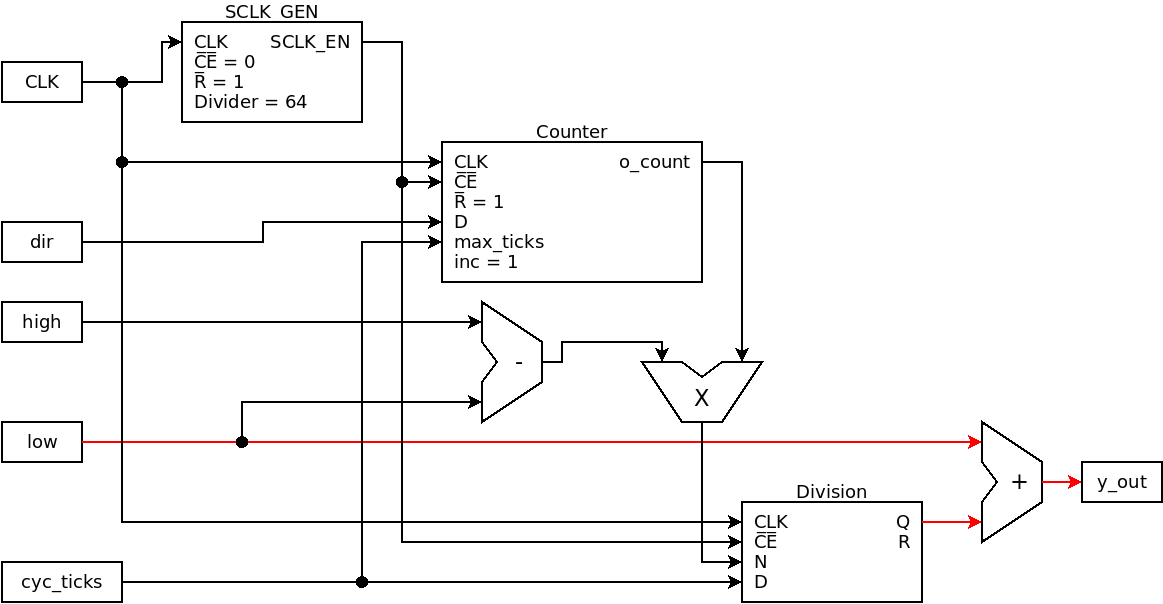
\includegraphics[scale=0.28]{ramp_step3}
  \end{figure}
\end{frame}

\begin{frame}{Komponenten - Zick-Zack}
  \begin{itemize}
    \item Zählrichtung wird mit Komperatoren geregelt
    \item halbe Zykluszeit (\emph{cyc\_ticks} um ein Bit nach rechts geschoben)
  \end{itemize}
  \begin{figure}
    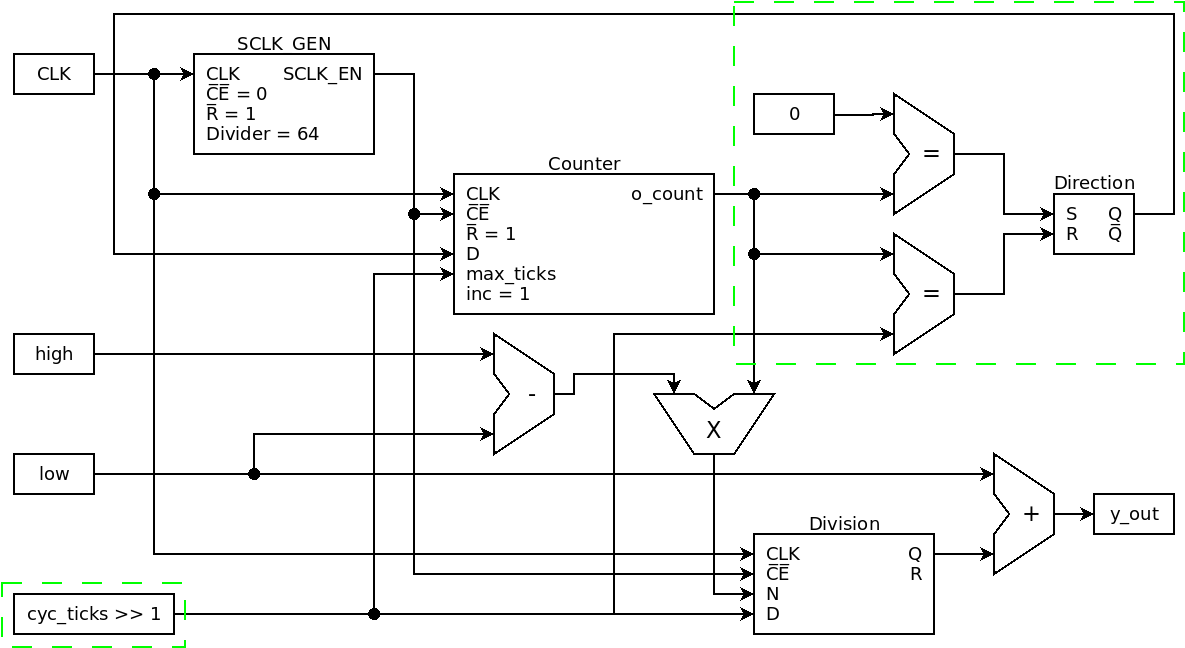
\includegraphics[scale=0.28]{zigzag}
  \end{figure}
\end{frame}


\section{Funktionstest}
\begin{frame}{Komponenten - Funktionsbausteine}
  
\end{frame}
\begin{frame}{Sources}
 
\printbibliography[title={Sources},heading=bibintoc]
\end{frame}

\end{document}